\chapter{Content-based image retrieval}
\label{ch:content_based}

Image retrieval and image indexing has been an active research field since the 1970s. In the 1978 (\cite{tamura1978textural}) a group of researchers proposed a system for retrieving textures based on the example texture. Since then, a wide range of techniques for image retrieval were presented. Traditional approaches included manual annotation of the images by textual or numerical metadata. The user could then formulate a query against these annotations to retrieve relevant images. This approach is often referred to as Concept-based image retrieval or meta-data search.

There are several drawbacks to the textual or numerical annotations. First of all, extensive human annotations are often needed to provide rich data for filtering. Including also spatial information of the objects takes more resources than only writing down present objects in the image. Furthermore, the images often include too many details (i.e. type, color, or shape of the objects), which may be impossible to comprehend by manual annotations.  The annotations may not even represent a stable truth. With a different annotator, the annotations may include different details/objects, which were perceived differently. When user searches for an image, she has to know the exact terms the annotators used in order to be able to retrieve the images they want. As the last problem, we pose with human annotations is the scalability. As the amount of information increases every second, there is no human capability to hand process all the examples.

During the 1990s, content-based image retrieval (CBIR) emerged (trend study from \cite{datta2008image}). In the CBIR approach, the images are indexed by features directly derived from their visual content using automatic or semi-automatic image processing techniques. Such indexing lacks building blocks (for example verbal description), on the other hand, provides low-level feature information about the whole images or its regions. The attributes of images are complex functions of regions of the image or the whole image.

CBIR has received considerable research interest in the last decades. With the advancement in Deep Learning, a new pool of possible complex functions to describe the images emerged. In our approaches, we use pre-trained neural networks to extract features. Based on these features, we implemented and evaluated several approaches to the CBIR task.

Presented techniques focus on the known-item search task. An alternative could be an Ad Hoc search, where the goal is to retrieve all relevant items to the query. Known-item search task rather works with retrieving a known item from the dataset.

Following this chapter, we continue with specifics of the individual approaches, we present. Here we formulate the task and the goal.

\section*{Task formulation and evaluation}

As our inputs we have a dataset of images and the target image (the image we look for). Since we work with known-item search task, we know that a target image is also present in the dataset. Our goal is to order the items in the database in a way, that the target image has the lowest rank. Alternatively said, if we order based on the similarity, we aim for the query and the target image to have the highest similarity. We refer to the position of our target image $t$ in ranked results as $rank_t$.
\todo[inline]{pozice obrazku v tomto usporadani je rank t vzhledem ku q je tolko}
\todo[inline]{we aim fot the query to have the highest similarity with the target image, good rank}
\todo[inlline]{v grafe, na x ovu os dat rank, popisat rank ... }
\todo[inlline]{\% of searched target images up to a given rank}
\todo[inline]{pripominame ze pozia obrazku v usporiadani oznacujeme ako rank}

Our goal is to develop a technique, which minimises the rank of the target image. In the following chapters we aim to test two different possibilities for query description.

We also provide a numerical comparison of the performance of different setups. To provide a comparison we a \emph{Rank of searched item}. The graphs shows the amount of the queries solved in a given rank. In all graphs an x-axis \todo{jednotky databaze a rank is represented as a percentage of the dataset} . The amount of queries solved is also expressed as the percentage.

\todo[inline]{nedava zmysel ten odstavec, krivka vyznacuje nie obsahuje, oznacuje mnozstvo dotazov up to a given rank}


We use a figure \ref{fig:mobilenet_whole_image_example} as an example to explain the graphs we use for evaluation of the performance of the system. In this specific case for 90\% of the annotated collages (queries), the target image was ranked in the first 50\% of the dataset. This can be also said in other words, that in 90\% of cases by stating a query we were able to eliminate half of the dataset as unrelated. We can also notice a steep curve in the beginning. It shows that 70\% of the collages had the target image ranked in the first 10\% of the dataset. We can see that this particular system worked well for 70\% of the collages well, but struggled to solve the rest.

\begin{figure}
    \centering
    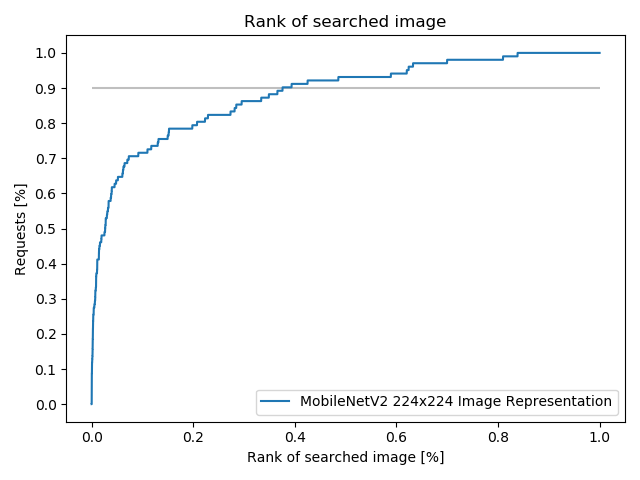
\includegraphics[width=0.8\linewidth]{img/mobilenet_whole_image.png}
    \caption{Performance of MobileNetV2 on annotated collages}
    \label{fig:mobilenet_whole_image_example}
\end{figure}

For these evaluations we use annotated queries. We described them in the section \ref{s:dataset}.